\documentclass[11pt]{article}

% Variable for HW number & name:
\newcommand{\class}{Stats 305c}
\newcommand{\hwnum}{4}
\newcommand{\quarter}{Spring 2026}

% Packages
\usepackage[margin=1in]{geometry}             
\geometry{letterpaper}                  
\usepackage{graphicx}
\usepackage{physics}
\usepackage{amsmath, amssymb, amsthm}
\usepackage{hyperref, multicol}
\hypersetup{colorlinks=false, allcolors=blue}
\usepackage[shortlabels]{enumitem}
\usepackage{bbm}
\usepackage{float}

% Commands for distributions
\newcommand{\Bern}{\mathrm{Bern}}
\newcommand{\Bin}{\mathrm{Bin}}
\newcommand{\HGeom}{\mathrm{HGeom}}
\newcommand{\Geom}{\mathrm{Geom}}
\newcommand{\FS}{\mathrm{FS}}
\newcommand{\Pois}{\mathrm{Pois}}
\newcommand{\Unif}{\mathrm{Unif}}
\newcommand{\Expo}{\mathrm{Expo}}
\newcommand{\Beta}{\mathrm{Beta}}
\newcommand{\Gam}{\mathrm{Gamma}}
\newcommand{\Logistic}{\mathrm{Logistic}}
\newcommand{\Nml}{\mathcal{N}}
\newcommand{\Lyap}{\mathrm{Lyap}}
\newcommand{\Lind}{\mathrm{Lind}}
\newcommand{\Rademacher}{\mathrm{Rademacher}}

% Commands for Var, Cov, Cor, etc.
\newcommand{\E}{\mathbb{E}}
\renewcommand{\P}{\mathbb{P}}
\newcommand{\Hcal}{\mathcal{H}}
\newcommand{\Var}{\mathrm{Var}}
\newcommand{\Cov}{\mathrm{Cov}}
\newcommand{\Cor}{\mathrm{Cor}}
\newcommand{\indi}{\mathbbm{1}}

% Commands for convergence
\newcommand{\toprob}{\xrightarrow{P}}
\newcommand{\todist}{\xrightarrow{D}}
\newcommand{\toas}{\xrightarrow{a.s.}}
\newcommand{\tolaw}{\xrightarrow{\mathcal{L}}}

% Commands for mathbb
\newcommand{\R}{\mathbb{R}}
\newcommand{\N}{\mathbb{N}}
\newcommand{\F}{\mathcal{F}}
\newcommand{\Q}{\mathbb{Q}}
\newcommand{\Z}{\mathbb{Z}}
\newcommand{\C}{\mathbb{C}}

% Setup for tcolorbox
\usepackage[most]{tcolorbox}
\tcbset{colback=green!5, colframe=green!75!black}

% Paragraph settings
\setlength{\parindent}{0pt}
\setlength{\parskip}{1.25ex}

% Solution environment
\newenvironment{sol}
    {\begin{tcolorbox}[breakable, pad at break*=1mm, parbox=false]
    }
    {
    \end{tcolorbox}
    }
    
% Page headers
\usepackage{fancyhdr}
\pagestyle{fancy}
\lhead{Kenny Gu and Scott Hwang}
\rhead{\class, Milestone \hwnum}

\newcommand{\noin}{\noindent}

% Indep symbol
\DeclareSymbolFont{symbolsC}{U}{txsyc}{m}{n}
\DeclareMathSymbol{\indep}{\mathrel}{symbolsC}{121}

% Document info
\title{\class\ Milestone \hwnum}
\author{Kenny Gu}
\date{April 2026}
                        
\begin{document}

\section{Recap}

This week, we continued refining our model. We begin by recalling that, in our last milestone, most of our geospatial models for predicting campaign contributions per zip code did not perform well on test data, relative to baseline null models (e.g., OLS or simply the train mean). On the other hand, when we shifted to predicting the difference in log campaign contributions per zip code (between the 2020 and 2022 cycles), we saw moderate improvements in test accuracy. However, we note that the improvements were still far less than ideal (e.g., test MSE of 3.30 vs. 3.24 for the train mean model vs our geospatial Bayesian model). Additionally, one can easily see that the posterior predictive samples do not seem to match particularly well:
\begin{figure}[h]
    \centering
    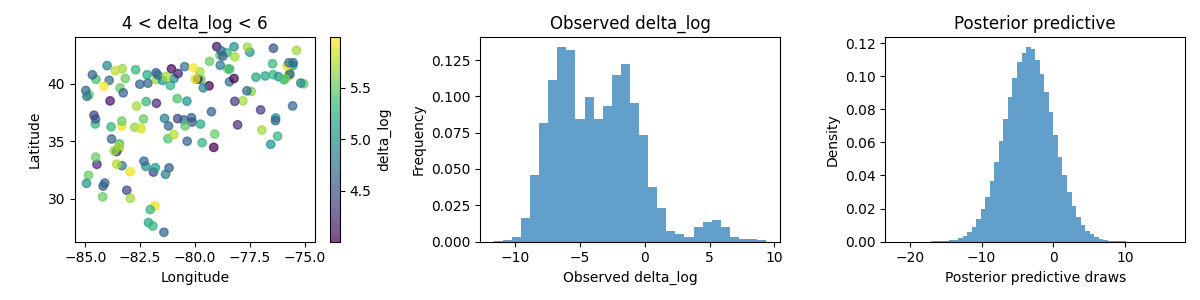
\includegraphics[width=0.8\linewidth]{../posterior_check_milestone3/posterior_predictive_check.png}
\end{figure}

In particular, we see that there appears to be an additional mode around 5 that is not matched in our posterior predictive distribution. On the left-most plot, we plot these zip codes that roughly correspond to this model: it doesn't seem like there is a clear spatial component (which rules out factors like state-level differences). 

\section{New modeling and methods}

In an attempt to improve our overall model performance, we instead fit models that include other covariates, including education covariates (proportion of adult population with a college degree or higher) and election covariates (including $\indi[\text{Senate election in 2022}] - \indi[\text{Senate election in 2020}]$). Additionally, rather than trying to predict the difference, we reframe our problem by using (log) contributions in 2020 as a covariate, rather than as part of our outcome. Finally, we also fit our model with a Mat\'ern 3/2 kernel, which we believe should allow for greater nonsmoothness in the spatial correlations.

We also attempt to fit our model to more observations: this time, we include 2000 data points sampled at random from the Eastern United States in our training set. One challenge, however, is that the model as written is now computationally intractable (at least locally on our machines, in the allotted time). Therefore, we considered two potential routes. At first, we considered the bootstrap method from Byers and Gill: however, we believe that the bootstrap method samples points that are very far away from one another, which leads to poor estimation of the relatively local effects. Therefore, we turned to the Vecchia approximation, which roughly approximates the likelihood of a Gaussian process by the product of likelihoods in local neighborhood (for this reason, it is also commonly referred to as a \textit{nearest neighbors Gaussian process method}). 

Here, we find much more success. Our trace plots and posterior draws are depicted in the figure below.
Our model is fit relatively efficiently (running in a little over three hours), and the trace plots seem to suggest convergence. Importantly, as opposed to the Bayesian model we ran last week, the plots this week suggest that the priors we use are suitable --- we no longer have the noise-related posteriors (e.g., related to the spatial kernel and nugget) simply hitting the maximum of the support of our prior.

In addition, we also build on papers in the related literature that use \textit{gravity models}, which try to model cash \textit{flows} between different areas (here, between zip codes and states) based on various covariates and distances (between contribution source and destination). However, as depicted below, we only see very marginal improvements over the null model (the train sample mean). \textcolor{red}{add details }


Fitting a simple linear model to these covariates suggests that the improvement in test MSE from last week is likely due to the explanatory power of these new covariates, not the spatial data. In fact, it seems that the Bayesian geospatial model does \textit{worse}, both compared to a OLS linear fit and to a Bayesian linear model (where the priors on the linear coefficients match but zip codes are modeled as conditionally independent draws).

\begin{figure}[h]
    \centering
    \makebox[\textwidth][c]{%
        \begin{minipage}[t]{0.58\textwidth}
            \centering
            \vspace{-10em}
            \begin{tabular}{lc}
            \hline
            Method & Test MSE \\
            \hline
            Train sample mean & 3.406 \\
            Model from last week & 3.245 \\
            Gravity model & \textcolor{red}{add MSE} \\
            OLS with all covariates above & 1.163 \\
            Bayesian geospatial model above & 1.204 \\
            Bayesian linear model & 1.163
            \end{tabular}
        \end{minipage}\hspace{0.03\textwidth}%
        \begin{minipage}[t]{0.4\textwidth}
            \centering
            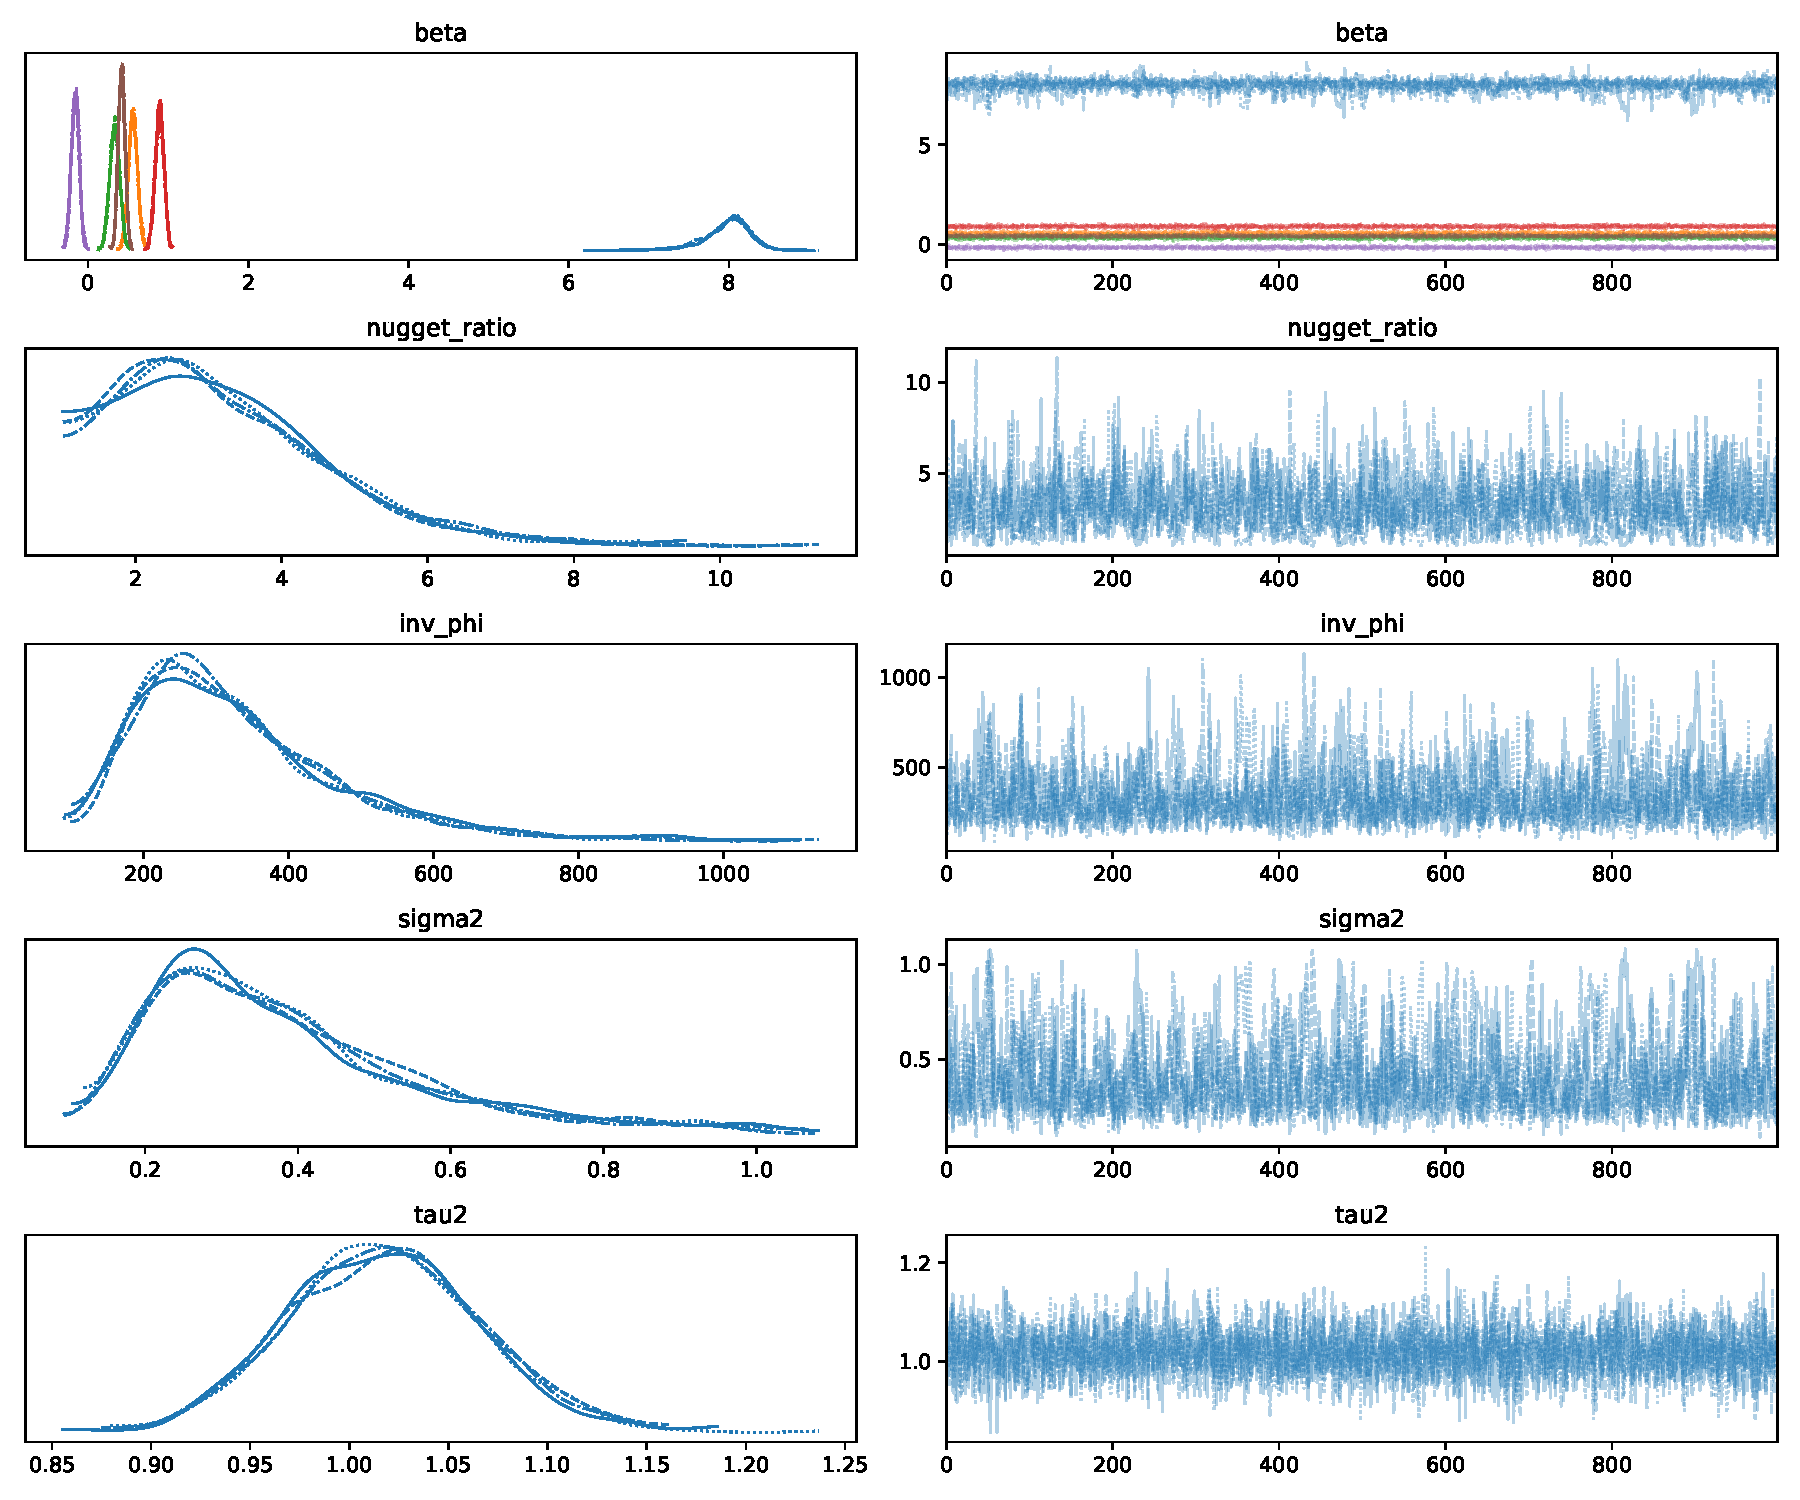
\includegraphics[width=\linewidth]{../nngp_trace.pdf}
        \end{minipage}%
    }
    % \caption{Test MSE comparison (left) and NNGP trace plots (right).}
\end{figure}


\section{Future directions}
The best model is still the simple OLS linear model, even though the semivariogram plots of the OLS residuals seem to suggest a strong spatial element. We note two potential reasons for this: (1) the Bayesian geospatial model adds greater complexity, which could lead to increased variance in our predictions, thus driving the MSE or (2) our geospatial modeling may not be sufficient (e.g., another modeling choice or fitting technique may be better suited).

To address (1), we might attempt to fit the model on a greater subset of the data or may attempt to perform some form of bagging. We could also attempt to predict contributions in other election cycles to increase our effective sample sizes. To address (2), we might attempt to increase the number of neighbors used in our Vecchia approximation or may attempt or to model spatial correlation in a more principled manner (perhaps reflecting artifial boundaries like state lines).

In the end, however, it might be that OLS (or Bayesian linear regression, so that we obtain uncertainty quantification as a byproduct) is simply the best technique for this task. It may be that the impact of covariates is sufficiently strong, that the data is sufficiently noisy/irregular, or that geospatial models are too complex to fit on the relatively limited data.




\newpage
\textbf{AI disclosure.} We used ChatGPT to help us implement and improve our MCMC samplers and to produce plots. All code was later manually reviewed by us.

\textbf{GitHub repository.} \href{https://github.com/kennethgu/stats305c-project/}{https://github.com/kennethgu/stats305c-project/}

% \bibliographystyle{plain} 
% \bibliography{milestone1}

\end{document}